% !TEX root = ./rapport.tex
% !TEX engine = latexmk -pdf
% !TEX buildOnSave = true
\documentclass[a4paper, 11pt, oneside]{article}

\usepackage[utf8]{inputenc}
\usepackage[T1]{fontenc}
\usepackage[french]{babel}
\usepackage{array}
\usepackage{shortvrb}
\usepackage{listings}
\usepackage[fleqn]{amsmath}
\usepackage{amsfonts}
\usepackage{fullpage}
\usepackage{enumerate}
\usepackage{graphicx}             % import, scale, and rotate graphics
\usepackage{subfigure}            % group figures
\usepackage{alltt}
\usepackage{url}
\usepackage{indentfirst}
\usepackage{eurosym}
\usepackage{color}
\usepackage[table,xcdraw,dvipsnames]{xcolor}
\usepackage{mdframed}
\usepackage{tikz}
\usepackage{float}
\usepackage{hyperref}

\hypersetup{
    colorlinks=true, % set to true to enable coloring of links
    linkbordercolor=white, % set the border color of internal links to white
    linkcolor=black % set the color of internal links to black
}

\renewcommand{\lstlistingname}{Extrait de Code}

\definecolor{mygray}{rgb}{0.5,0.5,0.5}
\newcommand{\coms}[1]{\textcolor{MidnightBlue}{#1}}

\lstset{
    language=C, % Utilisation du langage C
    commentstyle={\color{MidnightBlue}}, % Couleur des commentaires
    frame=single, % Entoure le code d'un joli cadre
    rulecolor=\color{black}, % Couleur de la ligne qui forme le cadre
    stringstyle=\color{RawSienna}, % Couleur des chaines de caractères
    numbers=left, % Ajoute une numérotation des lignes à gauche
    numbersep=5pt, % Distance entre les numérots de lignes et le code
    numberstyle=\tiny\color{mygray}, % Couleur des numéros de lignes
    basicstyle=\tt\footnotesize,
    tabsize=3, % Largeur des tabulations par défaut
    keywordstyle=\tt\bf\footnotesize\color{Sepia}, % Style des mots-clés
    extendedchars=true,
    captionpos=b, % sets the caption-position to bottom
    texcl=true, % Commentaires sur une ligne interprétés en Latex
    showstringspaces=false, % Ne montre pas les espace dans les chaines de caractères
    escapeinside={(>}{<)}, % Permet de mettre du latex entre des <( et )>.
    inputencoding=utf8,
    literate=
  {á}{{\'a}}1 {é}{{\'e}}1 {í}{{\'i}}1 {ó}{{\'o}}1 {ú}{{\'u}}1
  {Á}{{\'A}}1 {É}{{\'E}}1 {Í}{{\'I}}1 {Ó}{{\'O}}1 {Ú}{{\'U}}1
  {à}{{\`a}}1 {è}{{\`e}}1 {ì}{{\`i}}1 {ò}{{\`o}}1 {ù}{{\`u}}1
  {À}{{\`A}}1 {È}{{\`E}}1 {Ì}{{\`I}}1 {Ò}{{\`O}}1 {Ù}{{\`U}}1
  {ä}{{\"a}}1 {ë}{{\"e}}1 {ï}{{\"i}}1 {ö}{{\"o}}1 {ü}{{\"u}}1
  {Ä}{{\"A}}1 {Ë}{{\"E}}1 {Ï}{{\"I}}1 {Ö}{{\"O}}1 {Ü}{{\"U}}1
  {â}{{\^a}}1 {ê}{{\^e}}1 {î}{{\^i}}1 {ô}{{\^o}}1 {û}{{\^u}}1
  {Â}{{\^A}}1 {Ê}{{\^E}}1 {Î}{{\^I}}1 {Ô}{{\^O}}1 {Û}{{\^U}}1
  {œ}{{\oe}}1 {Œ}{{\OE}}1 {æ}{{\ae}}1 {Æ}{{\AE}}1 {ß}{{\ss}}1
  {ű}{{\H{u}}}1 {Ű}{{\H{U}}}1 {ő}{{\H{o}}}1 {Ő}{{\H{O}}}1
  {ç}{{\c c}}1 {Ç}{{\c C}}1 {ø}{{\o}}1 {å}{{\r a}}1 {Å}{{\r A}}1
  {€}{{\euro}}1 {£}{{\pounds}}1 {«}{{\guillemotleft}}1
  {»}{{\guillemotright}}1 {ñ}{{\~n}}1 {Ñ}{{\~N}}1 {¿}{{?`}}1
}

\begin{document}

\lstset{language=C, commentstyle={\color{blue}}, frame=single,
stringstyle=\color{magenta}}

\title{INFO0030: Projet 4, Mastermind}
\author{Groupe 10: Thomas Fraiponts, Martin Schins}
\date{Mai 2024}

\maketitle
\newpage

% !TEX root = ./rapport.tex
\section{Introduction}

À travers ce rapport, nous allons explorer l'architecture générale de notre code, en mettant en évidence les principaux concepts et leur interaction. Nous examinerons aussi les structures de données que nous avons développées, en discutant de leur pertinence et de leur coût. De plus, nous détaillerons les algorithmes que nous avons conçus pour gérer certaines fonctionnalités du jeu. Enfin, nous aborderons l'interface graphique, la gestion du SCM, la coopération au sein du groupe, les améliorations possibles et les enseignements tirés de cette expérience.
% !TEX root = ./rapport.tex

\section{Architecture générale du code}

Notre code suit le pattern modèle-vue-contrôleur (MVC) tel que vu au cours. Nous avons choisi de créer un modèle, une vue et un contrôleur pour le menu principal ainsi qu'un autre modèle-vue-contrôleur pour le jeu. Séparer le menu principal du jeu nous a permis de simplifier l'organisation et la structure du code. Il était alors facile d'ajouter un élément dans le menu sans devoir toucher à la création ou la gestion de la mémoire pour le jeu.
\\\\
La fenêtre "Abouts" qui affiche des informations sur le jeu et la fenêtre "End game" qui affiche si le joueur a gagné ou perdu en fin de partie ont été conservées dans le modèle-vue-contrôleur du jeu. En effet, dans leur cas, envisager de créer une vue et un contrôleur complexifierait la lecture du code et l'organisation de la vue et du contrôleur du jeu.

\subsection{Modèle}

Les pions de couleurs et les pions de résultat d'une combinaisons sont représentés grâce à des énumérations. Pour connaître le nombre de pions de couleur ou de pions de résultat nous plaçons en tout dernier dans les énumartions $NB\_PAWN\_COLORS$ et $NB\_FB\_COLORS$.
\begin{lstlisting}[language=C]
typedef enum{
    PAWN_BLUE,
    PAWN_CYAN,
    PAWN_GREEN,
    PAWN_ORANGE,
    PAWN_PURPLE,
    PAWN_RED,
    PAWN_YELLOW,
    PAWN_DEFAULT,
    NB_PAWN_COLORS
}PAWN_COLOR;
\end{lstlisting}

\begin{lstlisting}[language=C]
typedef enum{
    FB_BLACK,
    FB_WHITE,
    FB_DEFAULT,
    NB_FB_COLORS
}FEEDBACK_COLOR;
\end{lstlisting}

Le type opaque $modelMainMenu$ représente l'ensemble des données du menu principal. Il stocke le pseudo sauvegardé par le joueur, la validité de ce pseudo sans laquelle le joueur sera incapable de lancer une partie. Le role du joueur ainsi que le nombre de pions choisit pour la partie.

\newpage

De cette manière, l'ensemble des paramètres peuvent être configurés dans un premier temps par l'utilisateur dans le menu. Ces paramètres restent conservés tant que le jeu n'est pas complètement quitté, ce qui permet, par exemple, au joueur de ne pas devoir renseigner à nouveau son pseudo en retournant dans le menu principal.
\begin{lstlisting}[language=C]
struct model_main_menu_t {
   char pseudo[MAX_PSEUDO_LENGTH];
   bool validPseudo;
   ROLE role;
   unsigned int nbPawns;
};
\end{lstlisting}

Le type opaque $Combination$ représente une combinaison. Chacun des pions de la combinaison est renseigné dans un tableau $pawns$ et son résultat est stocké dans les champs $nbCorrect$ et $nbMisplaced$.
\begin{lstlisting}[language=C]
struct combination_t {
   unsigned int nbCorrect;
   unsigned int nbMisplaced;
   PAWN_COLOR *pawns;
};
\end{lstlisting}

Le type opaque $History$ représente l'historique des combinaisons proposées durant la partie. Les combinaisons sont stockées dans un tableau de $Combination$. $currentIndex$ est l'indice de la dernière combinaison dans le tableau de combinaisons.
\begin{lstlisting}[language=C]
struct history_t {
   unsigned int nbPawns;
   unsigned int nbCombinations;
   int currentIndex;
   Combination **combinations;
};
\end{lstlisting}

Le type opaque $Score$ représente une ligne de score dans le tableau des scores. Chaque ligne est composée d'un pseudo et d'une valeur de score.
\begin{lstlisting}[language=C]
struct score_t {
   char pseudo[MAX_PSEUDO_LENGTH];
   unsigned score;
};
\end{lstlisting}

Le type $SavedScores$ représente l'ensemble des scores renseignés dans le fichier texte. Cette structure nous permet de charger facilement l'ensemble des scores en créant un tableau de $Score$.
\begin{lstlisting}[language=C]
struct saved_scores_t {
   unsigned length;
   Score **savedScores;
};
\end{lstlisting}

Le type opaque $modelMastermind$ représente l'ensemble des données du jeu. On y copie les paramètres du menu principal tel que le pseudo, le role ainsi que le nombre de pions (plus précisément stocké dans l'historique). On y retrouve également la couleur sélectionnée, le proposition actuelle du joueur, la validité de la solution proposée, la solution de la partie, l'historique des combinaisons, le résultat du joueur vis à vis de la dernière combinaison proposée par l'ordinateur, le nombre de configurations créables, l'ensemble des configurations créables ainsi que le tableau de score.

\newpage

\begin{lstlisting}[language=C]
struct model_mastermind_t {
   ROLE role;
   char savedPseudo[MAX_PSEUDO_LENGTH];
   bool inGame;
   PAWN_COLOR selectedColor;
   Combination *proposition;
   bool validSolution;
   PAWN_COLOR *solution;
   History *history;
   FEEDBACK_COLOR *feedback;
   unsigned int nbConfigs;
   unsigned int lastConfigIndex;
   Combination **configs;
   SavedScores *save;
};
\end{lstlisting}
Le coût de cette approche augmente légèrement la complexité, car elle nécessite la définition de plusieurs structures de données. Cependant, elle rend le code plus modulaire et plus facile à gérer, ce qui, dans de nombreux cas, nous a permis d'ajouter et retirer facilement des fonctionnalités.

\subsection{View}
Les types opaques $viewMainMenu$ et $viewMastermind$ stockent l'ensemble des éléments affichés à l'écran qui ne permettent pas d'interactions avec l'utilisateur (i.e. tables, boxs, labels, boutons uniquement utiles à l'affichage d'une image...).

\begin{lstlisting}[language=C]
struct view_main_menu_t {
   ModelMainMenu *mmm;
   GtkWidget *window;
   GtkWidget *mainVBox;
   GtkWidget *pseudoHBox;
   GtkWidget *nbPawnsHBox;
   GtkWidget *logo;
   GtkWidget *pseudoLabel;
   GtkWidget *errorLabel;
   GtkWidget *nbPawnsLabel;
};
\end{lstlisting}

L'ensemble des pixbufs des images sont crées avant le lancement du menu ou du jeu. Dès lors, le programme ne s'interrompt pas soudainement en pleine partie lorsque que la création du pixbuf d'une image est impossible.  

Les boutons affichant l'historique des combinaisons ainsi que les boutons affichant l'historique des feedbacks sont quant à eux stockés dans des matrices de boutons.

\begin{lstlisting}[language=C]
struct view_mastermind_t {
   ModelMastermind *mm;
   unsigned int smallButtonSize;
   unsigned int bigButtonSize;
   unsigned int colorButtonSize;
   unsigned int propositionButtonSize;
   GdkPixbuf *winImage;
   GdkPixbuf *looseImage;
   GtkWidget *endGameWindow;
   GtkWidget *windowAbouts;
   GtkWidget *windowScore;
   GtkWidget *aboutsMainVBox;
   GtkWidget *scoreMainVBox;
   GtkWidget *aboutsLabel;
   GtkWidget *scoresTitleLabel;
   GtkWidget *scoresLabels[MAX_SCORE_DISPLAYED];
   GtkWidget *window;
   GtkWidget *mainVBox;
   GtkWidget *historyTable;
   GtkWidget *feedbackZoneHBox;
   GtkWidget *propositionHBox;
   GtkWidget *propositionControlHBox;
   GtkWidget *colorSelectionHBox;
   GtkWidget *scoreHBox;
   GdkPixbuf **colorImagePixbufs;
   GdkPixbuf **feedbackImagePixbufs;
   GtkWidget ***historyCombinations;
   GtkWidget ***historyFeedbacks;
   GtkWidget *scoreLabel;
};
\end{lstlisting}

\subsection{Contrôleur}

Les types opaques $controllerMainMenu$ et $controllerMastermind$ stockent l'ensemble des éléments affichés à l'écran qui permettent une ou plusieurs interactions avec l'utilisateur (i.e. boutons, sliders, boites d'entrée de texte, barre de menu...).

\begin{lstlisting}[language=C]
struct controller_main_menu_t {
   ModelMainMenu *mmm;
   ViewMainMenu *vmm;
   GtkWidget *pseudoEntry;
   GtkWidget *saveButton;
   GtkWidget *guesserButton;
   GtkWidget *proposerButton;
   GtkWidget *nbPawnsSlider;
   GtkWidget *playButton;
   GtkWidget *quitButton;
};
\end{lstlisting}

Le type opaque $menuBar$ nous permet de facilement créer une barre de menu sans alourdir le contrôleur du jeu. 

\begin{lstlisting}[language=C]
struct menu_bar_t {
   GtkWidget *bar;
   GtkWidget *menuGame;
   GtkWidget *menuHelp;
   GtkWidget *itemGame;
   GtkWidget *itemHelp;
   GtkWidget *itemMainMenu;
   GtkWidget *itemScore;
   GtkWidget *itemQuit;
   GtkWidget *itemAbouts;
};
\end{lstlisting}

Les boutons permettant au joueur de sélectionner une couleur, de créer une combinaison ou de créer un résultat sur une combinaison proposée par l'ordinateur sont stockés dans des tableaux de boutons. 

\begin{lstlisting}[language=C]
struct controller_mastermind_t {
   ControllerMainMenu *cmm;
   ModelMastermind *mm;
   ViewMastermind *vm;
   GtkWidget *aboutsOkayButton;
   GtkWidget *scoreOkayButton;
   MenuBar *menuBar;
   GtkWidget *applyButton;
   GtkWidget *resetButton;
   GtkWidget **colorSelectionButtons;
   GtkWidget **propositionButtons;
   GtkWidget **feedbackButtons;
};
\end{lstlisting}
% !TEX root = ./rapport.tex

\section{Algorithmes particuliers}

Notre algorithme, $determine\_feedback\_proposition$, nous permet de déterminer le résultat d'une combinaison proposée durant la partie. D'abord, nous initialisons des compteurs pour suivre le nombre d'occurrences de chaque couleur dans la proposition du joueur et dans la solution secrète. Cela nous permet de comparer les deux ensembles de pions par la suite.
\\\\
Ensuite, nous parcourons chaque pion de la proposition et chaque pion de la solution. Si un pion de la proposition est à la même position qu'un pion correspondant dans la solution, nous incrémentons le nombre de pions corrects. Sinon, nous mettons à jour les compteurs de couleur correspondants pour les pions mal placés.
\\\\
Et une fois que tous les pions ont été évalués, nous comparons les compteurs de couleur de la proposition et de la solution pour déterminer le nombre de pions mal placés. De cette manière, les pions mal placés sont correctement comptés même s'ils apparaissent plusieurs fois dans la proposition ou la solution.

\begin{lstlisting}[language=C]
void determine_feedback_proposition(ModelMastermind *mm, Combination 
*proposition, const PAWN_COLOR *solution) {
   assert(mm != NULL && proposition != NULL && solution != NULL);

   unsigned int nbColorsInProposition[NB_PAWN_COLORS];
   unsigned int nbColorsInSolution[NB_PAWN_COLORS];

   for(unsigned int i = 0; i < NB_PAWN_COLORS; i++){
      nbColorsInProposition[i] = 0;
      nbColorsInSolution[i] = 0;
   }

   for(unsigned int i = 0; i < mm->history->nbPawns; i++){
      if(proposition->pawns[i] == solution[i])
         proposition->nbCorrect++;
       
      else{
         nbColorsInProposition[proposition->pawns[i]]++;
         nbColorsInSolution[solution[i]]++;
      }
   }

   for(unsigned int i = 0; i < NB_PAWN_COLORS; i++){
      if(nbColorsInProposition[i] < nbColorsInSolution[i])
         proposition->nbMisplaced += nbColorsInProposition[i];
      else
         proposition->nbMisplaced += nbColorsInSolution[i];
   }
}
\end{lstlisting}

Notre algorithme $load\_scores$ nous permet de charger les scores enregistrés à partir d'un fichier texte. D'abord, nous vérifions que le chemin du fichier est valide. Ensuite, nous allouons de la mémoire pour stocker les scores chargés à partir du fichier. Nous utilisons notre structure savedScores qui nous permet de stocker facilement chacun des scores. 
\\\\
Si le fichier existe et peut être ouvert en lecture, nous le parcourons pour récupérer le nombre total de scores enregistrés. Ensuite, nous allouons de la mémoire pour stocker chaque score individuel, en lisant le pseudo et le score à partir du fichier et en les enregistrant dans notre structure de données. En cas d'échec de l'une de ces étapes, nous libérons toute la mémoire allouée et renvoyons NULL pour indiquer une erreur.
\\\\
Pour l'algorithme $write\_scores$, nous vérifions que les scores et le chemin du fichier sont valides. Ensuite, nous ouvrons le fichier en mode écriture. Si l'ouverture du fichier réussit, nous écrivons d'abord le nombre total de scores dans le fichier. Ensuite, nous parcourons chaque score et écrivons le pseudo et le score dans le fichier, ligne par ligne. Une fois tous les scores écrits, nous fermons le fichier. En cas d'échec de l'écriture ou de l'ouverture du fichier, nous affichons un message d'erreur et renvoyons un code d'erreur approprié.
\\\\
En utilisant ces deux algorithmes, nous pouvons facilement charger et sauvegarder les scores du jeu dans un fichier externe, ce qui permet de conserver les scores entre les sessions de jeu et de les partager aux différents joueurs.

\begin{lstlisting}[language=C]
SavedScores *load_scores(const char *filePath) {
   assert(filePath != NULL);

   SavedScores *save = malloc(sizeof(SavedScores));
   if(save == NULL)
      return NULL;

   if(access(filePath, F_OK) == 0){
      FILE *pFile = fopen(filePath, "r");
      if(pFile == NULL)
         return NULL;

      if(!fscanf(pFile, "%u\n", &save->length)){
         free(save);
         fclose(pFile);
         return NULL;
      }

      save->savedScores = malloc(save->length * sizeof(Score *));
      if(save->savedScores == NULL){
         free(save);
         fclose(pFile);
         return NULL;
      }

      for(unsigned i = 0; save->length > i; i++){
         save->savedScores[i] = malloc(sizeof(Score));
         if(save->savedScores[i] == NULL){
            for(unsigned j = 0; j < i; j++)
               free(save->savedScores[j]);

            free(save->savedScores);
            free(save);
            fclose(pFile);
            return NULL;
         }
         if(!fscanf(pFile, "%s %u\n", save->savedScores[i]->pseudo,
                    &save->savedScores[i]->score)){
            for(unsigned j = 0; j < i; j++)
               free(save->savedScores[j]);

            free(save);
            fclose(pFile);
            return NULL;
         }
      }
   } else{
      save->length = 0;
      save->savedScores = malloc(sizeof(Score *));
      if(save->savedScores == NULL){
         free(save);
         return NULL;
      }
   }

   return save;
}


int write_scores(SavedScores *scores, const char *filePath) {
   assert(scores != NULL && filePath != NULL);

   FILE *pFile = fopen(filePath, "w");
   if(pFile == NULL){
      fprintf(stderr, "Error while saving score");
      return -1;
   }

   fprintf(pFile, "%u\n", scores->length);

   for(unsigned i = 0; i < scores->length; i++){
      fprintf(pFile, "%s %u\n", scores->savedScores[i]->pseudo,
              scores->savedScores[i]->score);
   }

   fclose(pFile);
   return 0;
}
\end{lstlisting}
% !TEX root = ./rapport.tex
\newpage
\section{Interface graphique}

\subsection{Menu principal}

\begin{figure}[htbp]
    \centering
    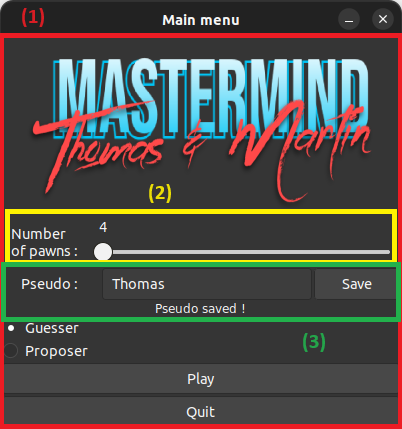
\includegraphics[width=0.5\textwidth]{main_menu.png}
    \caption{Fenêtre du menu principal.}
\end{figure}

La fenêtre du menu principal se décompose en une box verticale principale $(1)$ qui contient :
\begin{itemize}
    \item l'image du logo,
    \item $(2)$ une première box horizontale contenant le label $"Number~of~ pawns"$ ainsi que le slider permettant de sélectionner le nombre de pions de la partie (entre 4 et 8),
    \item $(3)$ une deuxième box horizontale contenant le label $"Pseudo:"$, une boite d'entrée de texte permettant au joueur de rentrer son pseudo ainsi qu'un bouton $Save$ pour le sauvegarder,
    \item un message informant de la validité et de la bonne sauvegarde du pseudo,
    \item deux boutons permettant de choisir le rôle de $Guesser$ (le joueur devine la combinaison aléatoire de l'ordinateur) ou $Proposer$ (l'ordinateur devine la combinaison du joueur),
    \item un bouton $Play$ permettant de lancer une partie,
    \item un bouton $Quit$ permettant de quitter le jeu.
\end{itemize}

\newpage
\subsection{Jeu}

\begin{figure}[htbp]
    \centering
    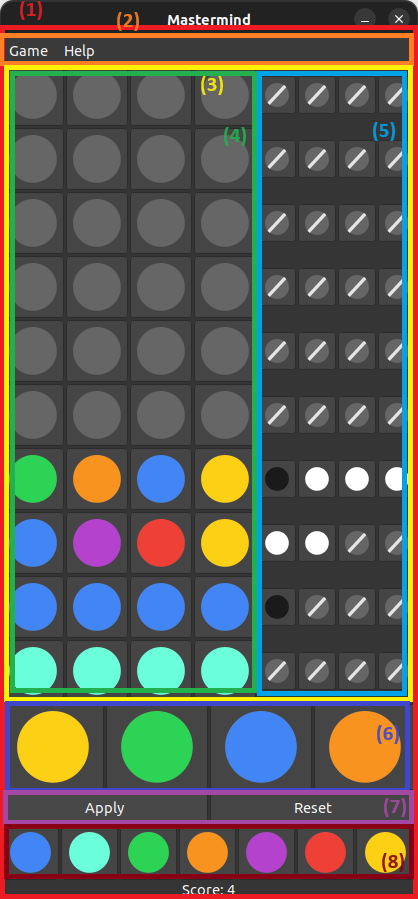
\includegraphics[width=0.414\textwidth]{game_guesser.png}
    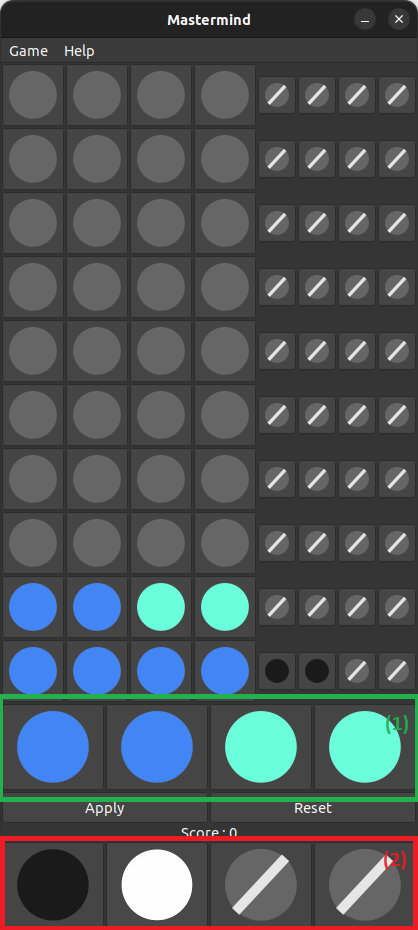
\includegraphics[width=0.4\textwidth]{game_proposer.png}
    \caption{Fenêtres de jeu ($Guesser$ à gauche et $Proposer$ à droite).}
\end{figure}

Les fenêtres de jeu en mode $Guesser$ et $Proposer$ partagent des éléments similaires. Les boites allant de $(1)$ à $(5)$ sur l'image de la fenêtre du jeu en mode $Guesser$ seront uniquement définies pour le mode $Guesser$ mais fonctionnent de la même manière en mode $Proposer$.
\\\\
La fenêtre de jeu se décompose en une box verticale principale $(1)$ contenant :

\begin{itemize}
    \item $(2)$ une barre de menu avec un bouton $Game$ et un bouton $Help$. $Game$ donne accès à un menu déroulant permettant les choix :
    \begin{itemize}
        \item $Main Menu$ qui permet de retourner au menu principal,
        \item $Score$ qui affiche une fenêtre répertoriant les 10 scores les plus élevés enregistrés,
        \item $Quit$ qui quitte complètement le jeu.
    \end{itemize}
    $Help$ donne accès à $Abouts$ qui ouvre une fenêtre affichant des informations à propos du jeu et de sa création.
    \item $(3)$ une table $Gtk$ organisant les boutons des boîtes $(4)$ et $(5)$. Il s'agit de l'historique de la partie.
    \item $(4)$ une matrice de boutons servant à l'affichage des images des pions de couleur. Ces lignes de boutons représentent les combinaisons proposées.
    \item $(5)$ une matrice de boutons servant à l'affichage des images des pions de feedback. Ces lignes de boutons sont les résultats correspondants aux combinaisons.
    \item[]
\end{itemize}

En mode de jeu $Guesser$, le tableau de boutons $(6)$ permet au joueur de créer une combinaison grâce aux différentes couleurs du tableau de boutons $(8)$. Une fois satisfait de la combinaison crée, le joueur peux proposer sa combinaison à l'aide du bouton $Apply$ $(7)$. Dans le cas contraire, le bouton $Reset~(7)$ permettera au joueur d'effacer sa combinaison. 
\\\\
En mode de jeu $Proposer$, l'affichage est, dans un premier temps, identique à celui du mode $Guesser$. Pour créer la combinaison que l'ordinateur devra trouver, le joueur utilise le même système que celui permettant de proposer des combinaisons en mode $Guesser$. Une fois la combinaison secrète proposée, elle est conservée dans la zone $(1)$ (sur l'image de la fenêtre du jeu en mode $Proposer$). Dès lors, l'ordinateur propose une combinaison qui est affichée dans l'historique et le joueur donne le résultat de la combinaison grâce aux boutons de la zone $(2)$. Pour faire apparaître des pions noirs ou blancs, le joueur devra cliquer plusieurs fois sur les boutons. Lorsque ce dernier est certain du résultat qu'il va donner à l'ordinateur, il le soumet via le bouton $Apply$.

\begin{figure}[htbp]
    \centering
    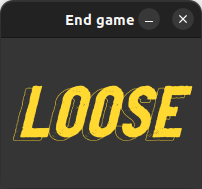
\includegraphics[width=0.2\textwidth]{loose.png}
    \caption{Fenêtre pop-up perdant.}
\end{figure}
En fin de jeu, une fenêtre pop-up apparaît affichant le résultat de la partie. Nous vous laissons le plaisir de découvrir l'affichage gagnant en ne vous dévoilant que le perdant.
% !TEX root = ./rapport.tex

\section{Gestion du SCM}

Au début de notre projet, l'utilisation de GitLab s'est avérée compliquée. Nous avons rencontré des difficultés lors de sa configuration et de sa prise en main, ce qui a considérablement ralenti le début du développement de notre projet. Une fois ces problèmes techniques résolus, nous avons constaté que les commits n'étaient pas suffisamment réguliers, ce qui a entraîné des difficultés à intégrer le travail de chacun. Nous avons également dû faire face à des conflits de fusion lors des pulls ce qui a entraîné des pertes de code.
\\\\
Cependant, à force d'utiliser et en comprenant davantage le fonctionnement de GitLab, nous avons commencé à travailler simultanément sur différentes parties du projet. Cela nous a permis de mieux organiser notre travail et de conserver des versions antérieures plus régulières du code. Au final, l'utilisation de GitLab nous a permis de rendre le processus de collaboration beaucoup plus fluide et rapide.
\\\\
Vous pouvez retrouver notre projet sur GitLab via le lien suivant :\\ \url{https://gitlab.uliege.be/Martin.Schins/info0030_groupe10}
% !TEX root = ./rapport.tex

\section{Coopération}

Pendant la réalisation de ce Mastermind, nous avons traversé différentes phases de coopération. D'abord, la répartition du travail s'est avérée être un exercice compliqué. Nous avons passé un temps considérable à discuter et à réfléchir sur la meilleure manière de répartir les tâches afin de tirer parti des forces et de tenir compte des faiblesses de chacun.
\\\\
Après plusieurs essais et erreurs, et grâce à l'aide précieuse des assistants à qui nous avons pu poser nos nombreuses questions, nous avons finalement réussi à comprendre pleinement le fonctionnement du pattern MVC et à l'intégrer dans notre projet. Nous avons donc opté pour travailler chacun de notre côté tout en continuant de nous informer mutuellement fréquemment.
\\\\
Pendant la réalisation du jeu, nous avons commencé à organiser des réunions plus fréquentes pour discuter des dernières fonctionnalités plus complexes du projet et pour résoudre les problèmes restants. De plus, nous avons progressivement eu recours à des sessions de travail en appel, ce qui nous a permis de mieux partager nos idées et de maintenir une motivation constante tout au long du projet.
\\\\
En fin de compte, la réalisation de ce Mastermind nous a permis de mieux comprendre l'importance du travail d'équipe et de la communication dans la réalisation de projets plus complexes. En exploitant les compétences de chacun, nous avons pu résoudre des problèmes que nous n'aurions peut-être pas su résoudre seuls. Ce projet a renforcé notre amitié ainsi que l'efficacité de notre travail de groupe.
% !TEX root = ./rapport.tex

\section{Suggestions d'améliorations}

Pendant le développement de notre Mastermind, nous avons envisagé plusieurs améliorations. Une idée principale était d'incorporer une ambiance sonore, comprenant une sélection de musiques de fond adaptées ainsi que des effets sonores pour accompagner les actions du joueur, comme des applaudissements pour une victoire ou des sons distincts lorsqu'on clique sur les différents boutons.
\\\\
De plus, nous avons envisagé d'offrir une personnalisation avancée de l'interface du jeu. Des réglages auraient été accessibles via une fenêtre de paramètres, permettant au joueur d'ajuster des éléments tels que la taille de la fenêtre de jeu, la couleur ou l'image de fond, ainsi que le volume de la musique et des effets sonores.
\\\\
Nous avons également pensé à l'ajout d'animations pour rendre le jeu plus dynamique et attrayant. Ces animations auraient inclus des transitions fluides entre le menu et le jeu, des effets visuels lors de la sélection des couleurs, et des animations spéciales pour marquer la découverte d'un pion bien positionné ou d'une combinaison correcte.
\\\\
De plus, nous avons envisagé l'implémentation de différents niveaux de difficulté pour offrir un défi adapté à tous les types de joueurs, allant des débutants en mode "proposer" préférant un feedback vérifié par l'ordinateur, aux joueurs expérimentés en mode "guesser" qui souhaitent limiter le nombre de combinaisons possibles.
\\\\
Enfin, nous aurions aimé créer un système de score plus réaliste qui fonctionnerait avec des bonus de vitesse de réponse ou encore des multiplicateurs de score liés à la difficulté du jeu. 
% !TEX root = ./rapport.tex

\section{Apprentissages}

La réalisation de ce Mastermind nous a appris l'importance cruciale d'avoir une vision structurée et un plan détaillé avant de se lancer dans le développement d'un projet de cette envergure. Nous avons réalisé que communiquer nos idées et s'expliquer nos raisonnements étaient un excellent moyen de garantir que tout ce qui a été prévu est raisonnablement envisageable.
\\\\
Le pattern MVC, bien qu'initialement complexe à mettre en place, est désormais beaucoup plus clair pour nous. Nous avons découvert qu'une fois établi, il permet d'ajouter et de supprimer des fonctionnalités sans compromettre la structure globale du code. 
\\\\
De plus, ce projet nous a permis de maîtriser GitLab, un outil indispensable pour nos futures années à l'Université.

\end{document}
